\documentclass{gts2012}

\usepackage{url}


% The packages graphicx, amssymb, and amsmath are already loaded via
% gts2012.cls

%----------------------- Macros and Definitions --------------------------

% Add all additional macros here, do NOT include any additional files.

% The environments theorem (Theorem), invar (Invariant), lemma (Lemma),
% cor (Corollary), obs (Observation), conj (Conjecture), prop 
% (Proposition), defini (Definition), and proof (Proof) are already defined 
% in the eurocg12.cls file. Add additional environments only if you REALLY 
% need them.

\newcommand\jPlex{\texttt{jPlex}\ }
\newcommand\javaPlex{\texttt{javaPlex}\ }

\newcommand{\VR}{\operatorname{VR}}
\newcommand{\LW}{\operatorname{LW}}
\newcommand{\image}{\operatorname{im}}
\newcommand{\preimage}{\operatorname{pre}}
\newcommand{\Hom}{\operatorname{Hom}}
\newcommand{\Ext}{\operatorname{Ext}}


%----------------------- Title -------------------------------------------

\title{javaPlex: a research platform for persistent homology}

\author{Andrew Tausz\thanks{ICME,
        Stanford University, {\tt atausz@stanford.edu}}
        \and
        Mikael Vejdemo-Johansson\thanks{School of Computer Science, University of St Andrews, Scotland
          , {\tt mvvj@st-andrews.ac.uk}}
        \and Henry Adams\thanks{Department of Mathematics,
        Stanford University, {\tt henrya@math.stanford.edu}}
        }

%------------------------------ Text -------------------------------------

\begin{document}
\maketitle

\begin{abstract}
The \javaPlex software package continues the Stanford tradition of software for persistent homology and cohomology computation. \javaPlex in particular is built with explicit aims for ease of use as a tool for research into computational topology, and is available under an open source license  with extensive source code documentation.

The main design aim in the construction of \javaPlex has been ease of extension -- lowering the threshold to implement new algorithms or insights from ongoing research into computational topology in a framework that provides most if not all current persistence algorithms in a single interface.

\end{abstract}

\section{Motivation and Design Goals}

The main reason for the existence of \javaPlex is to provide researchers in the area of topological data analysis a unified software library to support their investigations. With this in mind, the design goals for it are as follows:

\begin{itemize}
\item {\bf Support for new directions for research: } The main goal of the \javaPlex package is to provide an extensible base to support new avenues for research in computational homology and data analysis. While its predecesor \jPlex was very well suited towards computing simplicial homology, its design made extension difficult.
\item {\bf Interoperability: } \javaPlex can be run either as a Java application, or it can be called from any Java compatible language. Supported languages include Matlab, Jython and Processing.
\item {\bf Adherence to generally accepted software engineering practices: } As a means to realizing the first goal, the \javaPlex software package was designed and implemented with software engineering best-practices. Emphasis was placed on maintainability, modularity and reusability of the different parts of the code.
\end{itemize}

We refer the reader to~\cite{Carlsson_09} for a very readable introduction to the field of topological data analysis as well as the computational tasks involved.

\section{Availability and Licensing}

\javaPlex is an open source package, available through Google Code at \url{http://code.google.com/p/javaplex}. The \javaPlex package is issued under the New BSD License which is describe at \url{http://www.opensource.org/licenses/bsd-license.php}. 

\section{Related Platforms}

The two platforms similar in capability and spirit to \javaPlex are Dionysus and GAP persistence. Dionysus contains state-of-the-art implementations of the standard algorithms for persistent topology and topological data analysis. While Dionysus may have an edge in terms of computational speed (especially since it is written in C++), \javaPlex is written so that it is maximally accessible to newcomers to the field of computational topology. GAP persistence is a new package developed by one of the authors which presents similar algorithms in the context of a computer algebra package.

%\section{Architecture}
%The choice of architecture for the program library reflects the ambition to provide a platform for ongoing research with \javaPlex. 

\subsection{Overall Structure}

In a nutshell, the two main capabilities of \javaPlex are:
\begin{itemize}
\item Computation of the persistent homology of filtered chain complexes of finite vector spaces
\item Automated construction of filtered complexes from geometric data 
\end{itemize}

We expect most users of \javaPlex to go through the ``standard'' persistent homology pipeline: compute persistent simplicial homology of complexes constructed from point cloud data using Vietoris-Rips or witness complexes. The internal structure, however, anticipates and includes further extensions.



\section{Algebraic Background on Persistence Modules}

To compute the homological properties of a point cloud,
\cite{ELZ_02} introduced persistent homology, refined by
\cite{Carlsson_04}. Using one of a whole family of methods, the point
cloud induces a filtered simplicial complex, where the filtration
encodes distance data as increasing ``closeness'' data for the data
points in the point cloud.

\begin{figure}[h]
  \centering
  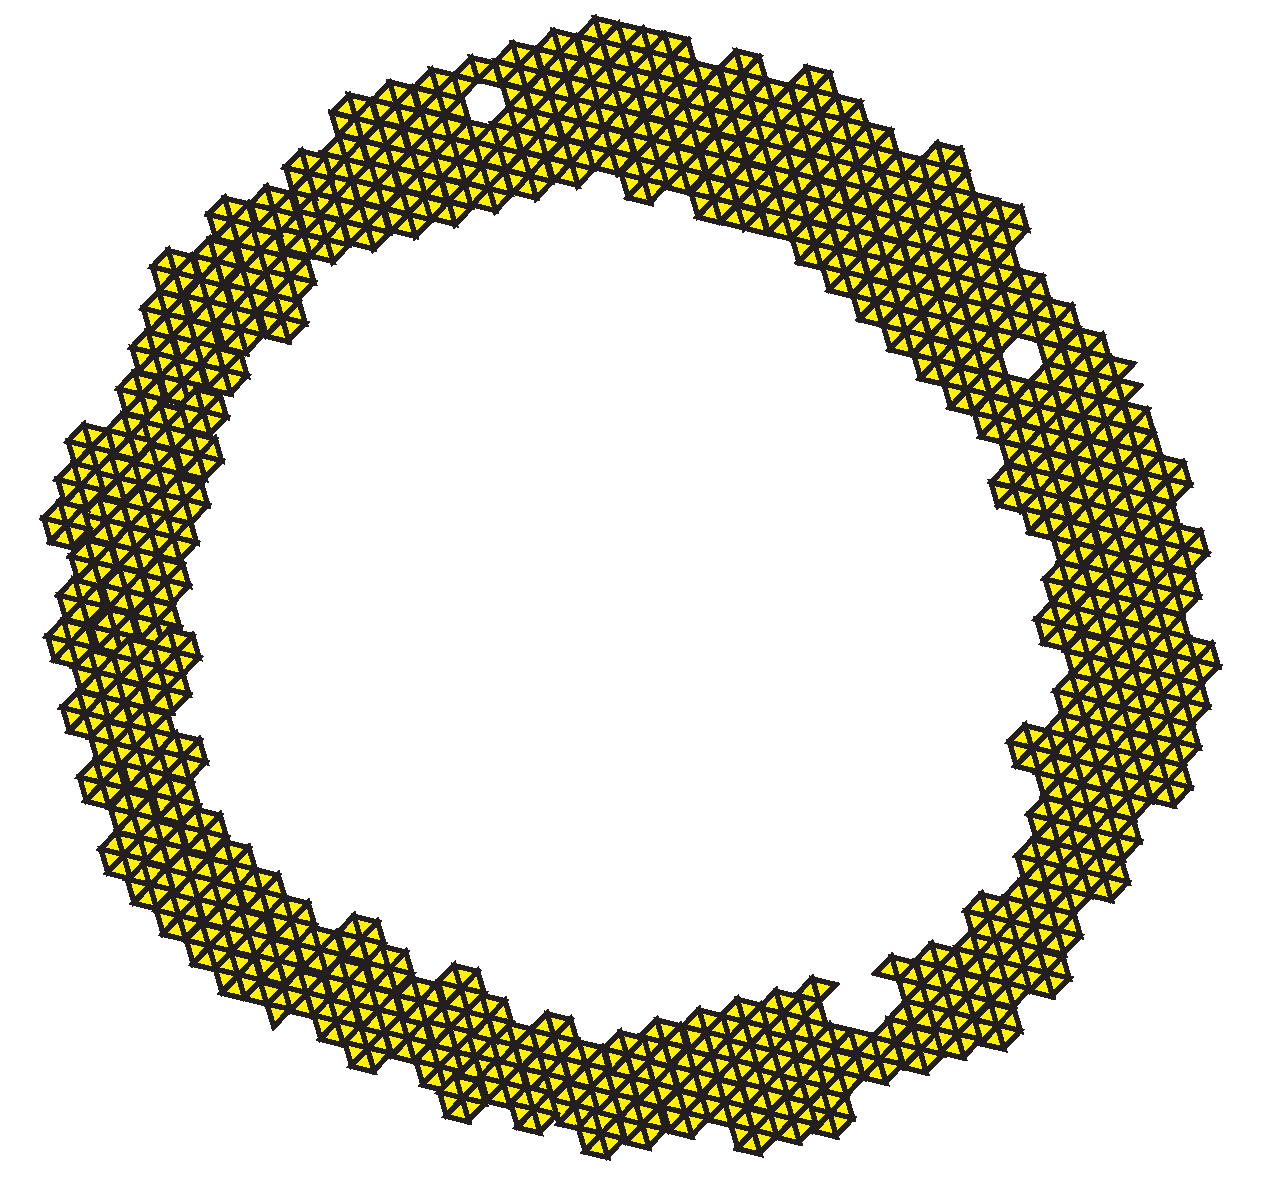
\includegraphics[width=0.4\textwidth]{images/perripstwo}
  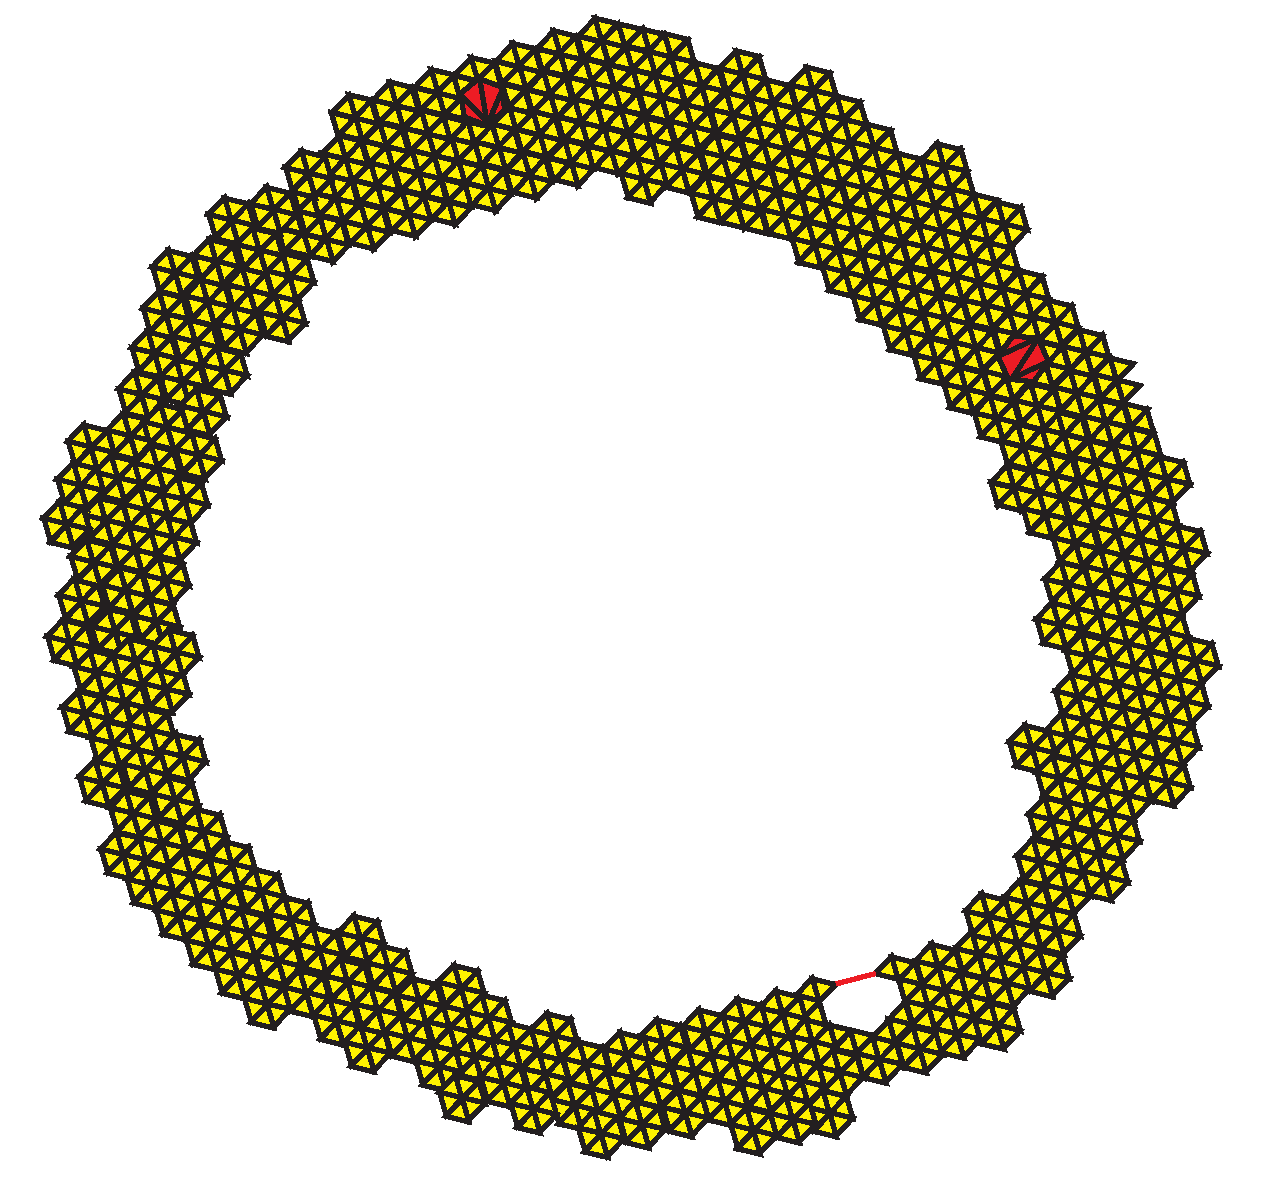
\includegraphics[width=0.4\textwidth]{images/perripsthree}
  \caption{Motivating the definition of persistence: the homology classes that survive from one stage to the next are more likely to be large and significant; all the small, potentially noise-induced classes exist in only one of these two stages.}
  \label{fig:betti3}
\end{figure}

Thus, from a point cloud, we acquire a filtered simplicial
complex. The homology of this with field coefficients is, since
homology is a functor, a linear diagram of vector spaces and linear
maps. 

Consider the situation in Figure \ref{fig:betti3}. To the left, we
have a hypothetical intermediate stage of a filtered simplicial
complex. The betti number at this stage, an indicator of the size of
the homology of a geometric object, would indicate a structure with
three holes. However, as the filtration continues, two of the three
detected holes are filled in, yielding the picture to the
right. However, the gap to the lower right ends up bridged, creating
two holes, both detected by the homology computation.

By a cursory inspection of the point cloud, we would be inclined to
say that the ``true'' number of relevant holes, or cycles, in the data
is just one -- and this one significant hole is characterized by the
homology class corresponding to the hole being in the image of the
inclusion map: the two superfluous cycles to the left vanish along the
map induced by the inclusion of simplicial complexes, and the
superfluous cycle to the left was not present before this induced
map.

This example motivates our definition of a \emph{persistent homology class}
with life time starting at the filtration stage $p$ and
\emph{persisting} through to filtration stage $q$ as an equivalence
class of cycles in the simplicial complex $\Sigma_p$ modulo boundaries
from the simplicial complex $\Sigma_q$.

%% NOTE to Andrew: if you want the paper to discuss zig-zag, this is
%% a good place to comment about how zig-zag modifies these
%% definitions.

The dimensions of such persistent homology groups are captured as
\emph{betti barcodes}, in which a line is drawn parallel to the
$x$-axis, from $p$ to $q$ for any basis element in this
$H^{p,q}_*(\Sigma_*)$. Similarly, a \emph{persistence diagram}
captures the same information, with each basis element corresponding
to the point $(p,q)$ in the plane. We view as significant features
those that are described by long intervals, or equivalently those with
a long distance from the $x=y$ diagonal in the persistence diagram.

As demonstrated in \cite{Carlsson_04}, the sequential diagrams of
linear vector spaces and linear maps
\[
V_0 \xrightarrow{i_0} V_1 \xrightarrow{i_1} \dots 
\]
corresponding to the homology of a filtered simplicial complex
correspond through an equivalence of categories to graded modules over
$\mathbb{F}[x]$, the polynomial ring in one variable. The equivalence
is by sending the diagram above to the vector space $\bigoplus_k V_k$,
and introducing an action of $x$ on this vector space by $x\cdot v=i_k(v)$
for $v\in V_k$.

The equivalence carries a long way: the chain complex of a filtered
simplicial complex is a filtered chain complex, which fits into this
model too, by making each stage correspond to the corresponding
filtration stage. Thus, the homology of a filtered simplicial complex
becomes a process entirely internal to the category of graded $\mathbb{F}[x]$-modules.

It should be noted that these modules are graded in two useful ways. One grading
comes from the filtration, setting $|v|=k$ for a basis element $v$ if
$v\in V_k/V_{k-1}$. Another comes from the dimension: $|v|=k$ if $v$
is a simplicial $k$-chain.


% \begin{itemize}
% \item Maybe the best person to write this would be Mikael or Gunnar??
% \item need to mention grading by filtration index vs grading by dimension
% \end{itemize}

\section{Filtered Complex Generation}

As mentioned in the abstract, the primary function of \javaPlex is the construction of filtered chain complexes of vector spaces associated to actual point cloud datasets. The motivation for such constructions is that they provide a persistent model of the dataset in question across all scales. \javaPlex currently supports the construction of two main types of filtered simplicial complexes: the Vietoris-Rips and lazy-witness constructions. To begin, suppose that we have a finite metric space $(\mathcal{X}, d)$. In practice, it is possible that $\mathcal{X}$ is a set of points in Euclidean space, although this is not necessary.

\subsection{The Vietoris-Rips Construction}
We define the filtered complex $\VR(\mathcal{X}, r)$ as follows. Suppose that the points of $\mathcal{X}$ are $\{x_1, ... x_N\}$, where $N = |\mathcal{X}|$. The Vietoris-Rips complex is constructed as follows:

\begin{itemize}
\item {\bf Add points:} For all points $x \in \mathcal{X}$, $x \in \VR_0(\mathcal{X}, 0)$
\item {\bf Add 1-skeleton:} The 1-simplex $[x_i, x_j]$ is in $\VR_1(\mathcal{X}, r)$ iff $d(x_i, x_j) \leq r$
\item {\bf Expansion:} We define $\VR(\mathcal{X}, r)$ to be the maximal simplicial complex containing $\VR_1(\mathcal{X}, r)$. That is, a simplex $[x_0, .. x_k]$ is in $\VR(\mathcal{X}, r)$ if and only if all of its edges are in $\VR_1(\mathcal{X}, r)$.
\end{itemize}

An extensive discussion on algorithms for computing the Vietoris-Rips complex can be found in \cite{Zomorodian}. The \javaPlex implementation is based on the results of this paper.

\subsection{The Lazy-Witness Construction}
The fundamental idea behind the lazy-witness construction is that a relatively small subset of a point cloud can accurately describe the shape of the dataset. This construction has the advantage of being more resistant to noise than the Vietoris-Rips construction. An extensive discussion about it can be found in \cite{Witness}. 

The lazy-witness construction starts with a selection of landmark points, $\mathcal{L} \subset \mathcal{X}$ with $|\mathcal{L}| = L$. One possibility is to simply choose a random subset of $\mathcal{X}$. Another possibility is to perform a sequential max-min selection: An initial point $l_0$ is selected, and then we inductively select the point $l_k$ which maximizes the minimum distance to all previously generated points. This max-min construction tends to produce more evenly spaced points than the random selection. Again we refer the reader to \cite{Witness} for a more detailed discussion, as well as empirical results supporting these claims.

This construction is parameterized by a value $\nu$, which most commonly takes the values 0, 1, or 2. We also define the distance matrix $D$ to contain the pairwise distances between the points in $\mathcal{X}$. 

\begin{itemize}
\item {\bf Define $m_i$:} If $\nu = 0$, let $m_i = 0$, otherwise, define $m_i$ to be the $\nu$-th smallest entry in the $i$-th column of D
\item {\bf Add points:} For all points $l \in \mathcal{L}$, $l \in \LW_0(\mathcal{X}, 0, \nu)$
\item {\bf Add 1-skeleton:} The 1-simplex $[l_i, l_j]$ is in $\LW_1(\mathcal{X}, r, \nu)$ iff there exists an $x \in \mathcal{X}$ such that $\max(d(l_i, x), d(l_j, x)) \leq r + m_i$.
\item {\bf Expansion:} We define $\LW(\mathcal{X}, r, \nu)$ to be the maximal simplicial complex containing $\LW_1(\mathcal{X}, r, \nu)$. 
\end{itemize}

\section{Homology Computation}

At the core of the \javaPlex library is the set of algorithms that actually compute the homology of a filtered chain complex. Key references to background material regarding these algorithms can be found in \cite{Carlsson_04, Dualities}. Although we do not describe them in detail here, we note that the algorithms for computing persistent absolute/relative (co)homology can be formulated as matrix decomposition problems. The fundamental reason for this is the equivalence of category of persistent vector spaces of finite type, and the category finitely generated graded modules over $\mathbb{F}[t]$. This correspondence is described in \cite{Carlsson_04}. 

The homology algorithms are built in a way that is optimized for chain complexes implemented as \emph{streams}. By this we mean that a filtered chain complex is represented by a sequence of basis elements that are produced in increasing order of their filtration indices. Enforcing the constraint that all complexes must be implemented this way allows \javaPlex to perform the matrix decomposition operations in an efficient online fashion.

\section{Applications}

Although in principle \javaPlex can compute the persistent homology of arbitrary chain complexes of vector spaces, almost always these complexes arise from some sort of topological construction. Below we outline these different situations.

\subsection{Simplicial Homology}

This is the ``standard'' situation, which was also handled by previous versions in the Plex software family. Here, we have a filtered sequence of simplicial complexes $X_1 \subset X_2 \subset ... \subset X_n$, from which we define the vector space of chains, $C(X_i)$ consisting of formal sums of elements of $X_i$ with coefficients in the field $\mathbb{F}$.

In this case the boundary operator $\partial: C(X_i) \rightarrow C(X_{i-1})$ is the actual geometric boundary defined by
$$\partial([v_0, ..., v_n]) = \sum_i (-1)^i [v_0, ..., \hat{v_i}, ..., v_n]$$

\subsection{Cellular Homology}

In this case, $X = X_*$ is a filtered cell complex. This complex is formed by inductively adding $n$-cells to the $n-1$-skeleton, by the gluing maps 
$$\varphi_{\alpha}^n: S^{n-1} \rightarrow X_{d-1}$$
which map the boundaries of the $n$-cells $e_{\alpha}^n$ to the $n-1$ skeleton. Note that in the above, we use $n$ to denote the grading by dimension, and $d$ to denote the grading by filtration index.

The boundary operator then becomes 
$$\partial(e_{\alpha}^n) = \sum_{\beta} \deg(\varphi_{\alpha \beta}^n) e_{\beta}^{n-1}$$
where $\deg$ refers to the topological degree of a map.

Note that while \javaPlex is fully capable of computing the persistent homology of arbitrary cell complexes, the specification of such complexes are more tedious than simplicial complexes. Nevertheless they offer the user a parsimonious way of defining a wide class of topological spaces.

\subsection{Operations on Chain Complexes}

The abstraction away from geometric primitives allows \javaPlex to handle more general algebraic constructions using complexes. These include computations such as tensor products, hom complexes and mapping cylinders.

\section{Examples}

\subsection{Simplicial Homology}

In Figure \ref{lwtorus}, one can see an example of a filtered simplicial complex generated from points on a torus. As one moves from left to right, the filtration parameter, $r$, is increased yielding a more connected complex. In Figure \ref{lwtorusbarcodes} we show the persistence barcodes for the same shape. Note that the significant intervals corresponding to homological features that last for a long time in the filtration.

\begin{figure}
\centering
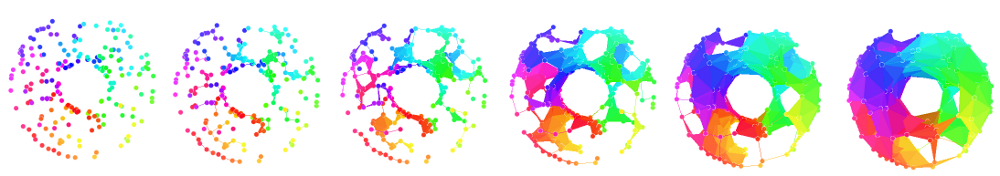
\includegraphics[width=0.9\textwidth]{images/tori_small.png}
\caption{Example of a Lazy-Witness complex generated from randomly sampled points on a torus.} \label{lwtorus}
\end{figure}

\begin{figure}
\centering
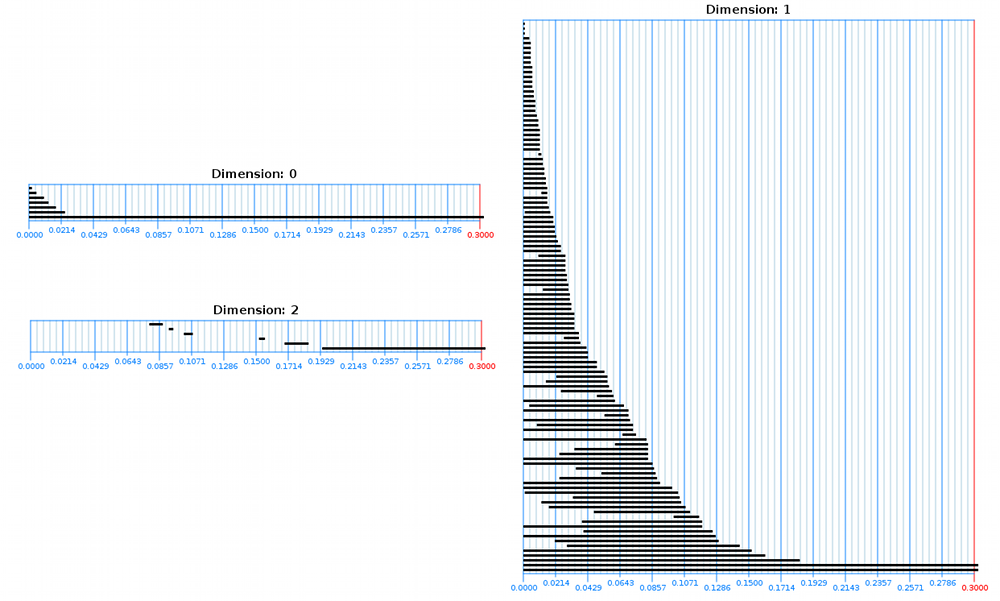
\includegraphics[width=0.9\textwidth]{images/barcodes_small.png}
\caption{Persistence barcodes for a lazy-witness filtration of random points on a torus. The parameters used were: $N = 1000$, $L = 300$, $r_{\max} = 0.3$. The inner and outer radii of the torus were 0.5 and 1, respectively. The max-min selection procedure was used to create the landmark set. Note that long intervals correspond to significant homological features, and short ones are most likely the result of noise. We can see that the number of significant intervals in each dimension equals the expected Betti number.} \label{lwtorusbarcodes}
\end{figure}

\subsection{Matlab Scripting Example - Cellular Homology}

In this section we show a brief Matlab session in which the cellular homology is computed for a Klein bottle over different coefficient fields. Essentially, this code examples constructs a cellular Klein bottle, initializes persistence algorithm objects over the fields $\mathbb{Z}/2\mathbb{Z}$, $\mathbb{Z}/3\mathbb{Z}$, and $\mathbb{Q}$, and computes the persistence intervals. We emphasize the fact that \javaPlex does not rely on Matlab in any way - it is merely being used as a scripting platform here.

\begin{verbatim}
% get the cellular sphere of the specified dimension
stream = examples.CellStreamExamples.getCellularKleinBottle();

% get cellular homology algorithm over Z/2Z
Z2_persistence = api.Plex4.getModularCellularAlgorithm(3, 2);
% get cellular homology algorithm over Z/3Z
Z3_persistence = api.Plex4.getModularCellularAlgorithm(3, 3);
% get cellular homology algorithm over Q
Q_persistence = api.Plex4.getRationalCellularAlgorithm(3);

% compute over Z/2Z - should give (1, 2, 1)
Z2_intervals = Z2_persistence.computeIntervals(stream)

% compute over Z/3Z - should give (1, 1, 0)
Z3_intervals = Z3_persistence.computeIntervals(stream)

% compute over Q - should give (1, 1, 0)
Q_intervals = Q_persistence.computeIntervals(stream)
\end{verbatim}
The output of this example is:
\begin{verbatim}
Z2_intervals =
Dimension: 2 [0, infinity)
Dimension: 1 [0, infinity), [0, infinity)
Dimension: 0 [0, infinity)
  
Z3_intervals =
Dimension: 1 [0, infinity)
Dimension: 0 [0, infinity)
 
Q_intervals =
Dimension: 1 [0, infinity)
Dimension: 0 [0, infinity)
\end{verbatim}
This is exactly what we expect, due to the presence of 2-torsion in the Klein bottle.



\begin{acknowledgments}
We would like to thank the reviewers for providing useful comments.
\end{acknowledgments}


%---------------------------- Bibliography -------------------------------

% Please add the contents of the .bbl file 

\footnotesize 
\bibliographystyle{abbrv}

\begin{thebibliography}{99}

\bibitem[Car09]{Carlsson_09}
Gunnar Carlsson, \emph{{Topology and data}}, Bulletin of the American
  Mathematical Society \textbf{46} (2009), no.~2, 255--308.

\bibitem[dSC04]{Witness}
Vin de~Silva and Gunnar Carlsson, \emph{{Topological estimation using witness
  complexes}}, Eurographics Symposium on Point-Based Graphics (M.~Alexa and
  S.~Rusinkiewicz, eds.), The Eurographics Association, 2004.

\bibitem[dSMVJ10]{Dualities}
Vin de~Silva, Dmitriy Morozov, and Mikael Vejdemo-Johansson, \emph{{Dualities
  in persistent (co)homology}}, Unpublished manuscript, 2010.

\bibitem[ELZ02]{ELZ_02}
Herbert Edelsbrunner, David Letscher, and Afra Zomorodian, \emph{Topological
  persistence and simplification}, Discrete Comput. Geom. \textbf{28} (2002),
  no.~4, 511--533, Discrete and computational geometry and graph drawing
  (Columbia, SC, 2001). {1949898 (2003m:52019)}

\bibitem[ZC05]{Carlsson_04}
Afra Zomorodian and Gunnar Carlsson, \emph{Computing persistent homology},
  Discrete Comput. Geom \textbf{33} (2005), 249--274.

\bibitem[Zom10]{Zomorodian}
A.~Zomorodian, \emph{Fast construction of the {V}ietoris-{R}ips complex},
  Computers \& Graphics \textbf{34} (2010), no.~3, 263 -- 271.


\end{thebibliography}

\end{document}

